\section{Final Velocity Model}
\eqref{eq:Totaltorquewithcurrentexpression} delivers the information needed to make a visual representation of the motor model. The input is the supply voltage, \si{V_m(s)} delivered to the motor and the output is the required torque, \si{\tau_m}, see \figref{fig:BlockDiagramDrivetrain}. The block representation of the system is used, when the system is to be simulated.

\begin{figure}[H]
	\centering
	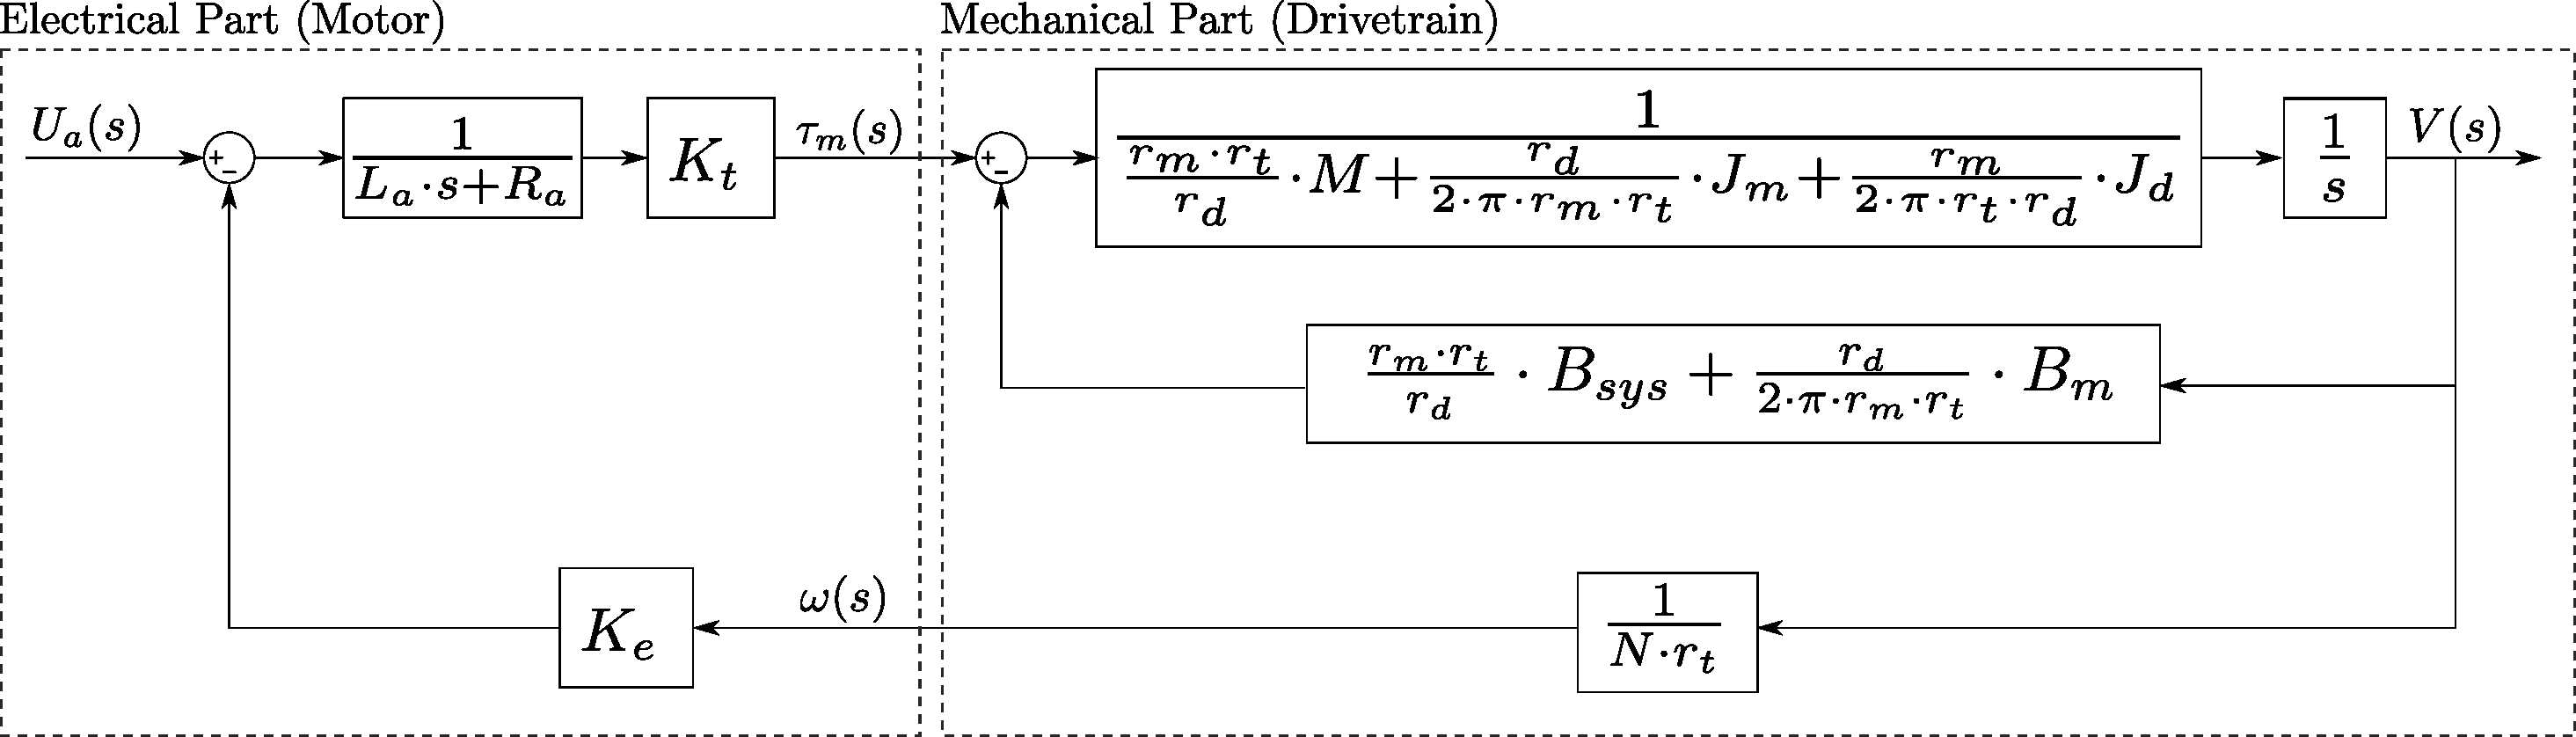
\includegraphics[width=\textwidth]{figures/totalVelocityModelDiagramComplicated.pdf}
	\caption{A block diagram of the combined drivetrain}
	\label{fig:BlockDiagramDrivetrain}
\end{figure}

The angular velocity received from the drivetrain, see \figref{fig:Velocitymodelplantopen}, is dependent on the total inertia of the system, and is necessary to ensure the motor is affected by the load.

A model of the electrical and mechanical part has been formed and a block representation of the motor's applied voltage and generated torque has been given. Next step is to model the drivetrain, which connects to the motor through the motor shaft.